\subsection{Strategy Pattern}

\subsubsection*{Problembeschreibung}

Es kann vorkommen, dass mehrere Varianten eines Algorithmus benötigt werden, welche alle eine einheitliche Schnittstelle bereitstellen. Je nach Kontext wird ein anderer Algorithmus benötigt. Die Algorithmen sollen dynamisch austauschbar sein, um deren flexiblen Einsatz zu ermöglichen und eine lose Kopplung zu gewährleisten. Eine Implementierung der Algorithmen-Varianten innerhalb der ausführenden Klasse, würde deren Komplexität deutlich erhöhen. Außerdem soll die Möglichkeit bestehen, in Zukunft weitere Algorithmen hinzuzufügen. Das \emph{Strategy-Pattern} kann die Übersichtlichkeit verbessern, wenn viele ähnliche Klassen existieren, die sich lediglich in ihrem verhalten unterscheiden. Weiterhin sollen Implementierungsdetails und Algorithmus-spezifische Daten vom Kontext abgekapselt werden. \cite{gamma_design_1995}

\subsubsection*{Lösung}

Wie in Abbildung \ref{fig:strategy-class} abgebildet, besitzt der Kontext (\code{Context}), welcher einen Algorithmus verwenden soll, eine Referenz auf eine Strategie (\code{Strategy}). Die konkrete Strategie (\code{ConcreteStrategy}) wurde dem Kontext zuvor durch den Anwender (\code{Client})\footnote{Der Anwender (\code{Client}) ist in der Regel eine weitere Klasse, welche den beschriebenen Mechanismus verwendet. Es handelt sich in aller Regel nicht um einen Menschen.\label{ftn:client}} mithilfe von \code{setStrategy} zugewiesen. Die konkrete Strategie realisiert die \code{Strategy}-Schnittstelle, sodass Kontext und konkrete Strategie lediglich lose gekoppelt sind. Jede Strategie stellt die Methode \code{execute} bereit, um den gekapselten Algorithmus auszuführen.

\begin{figure}[H]
	\centering
	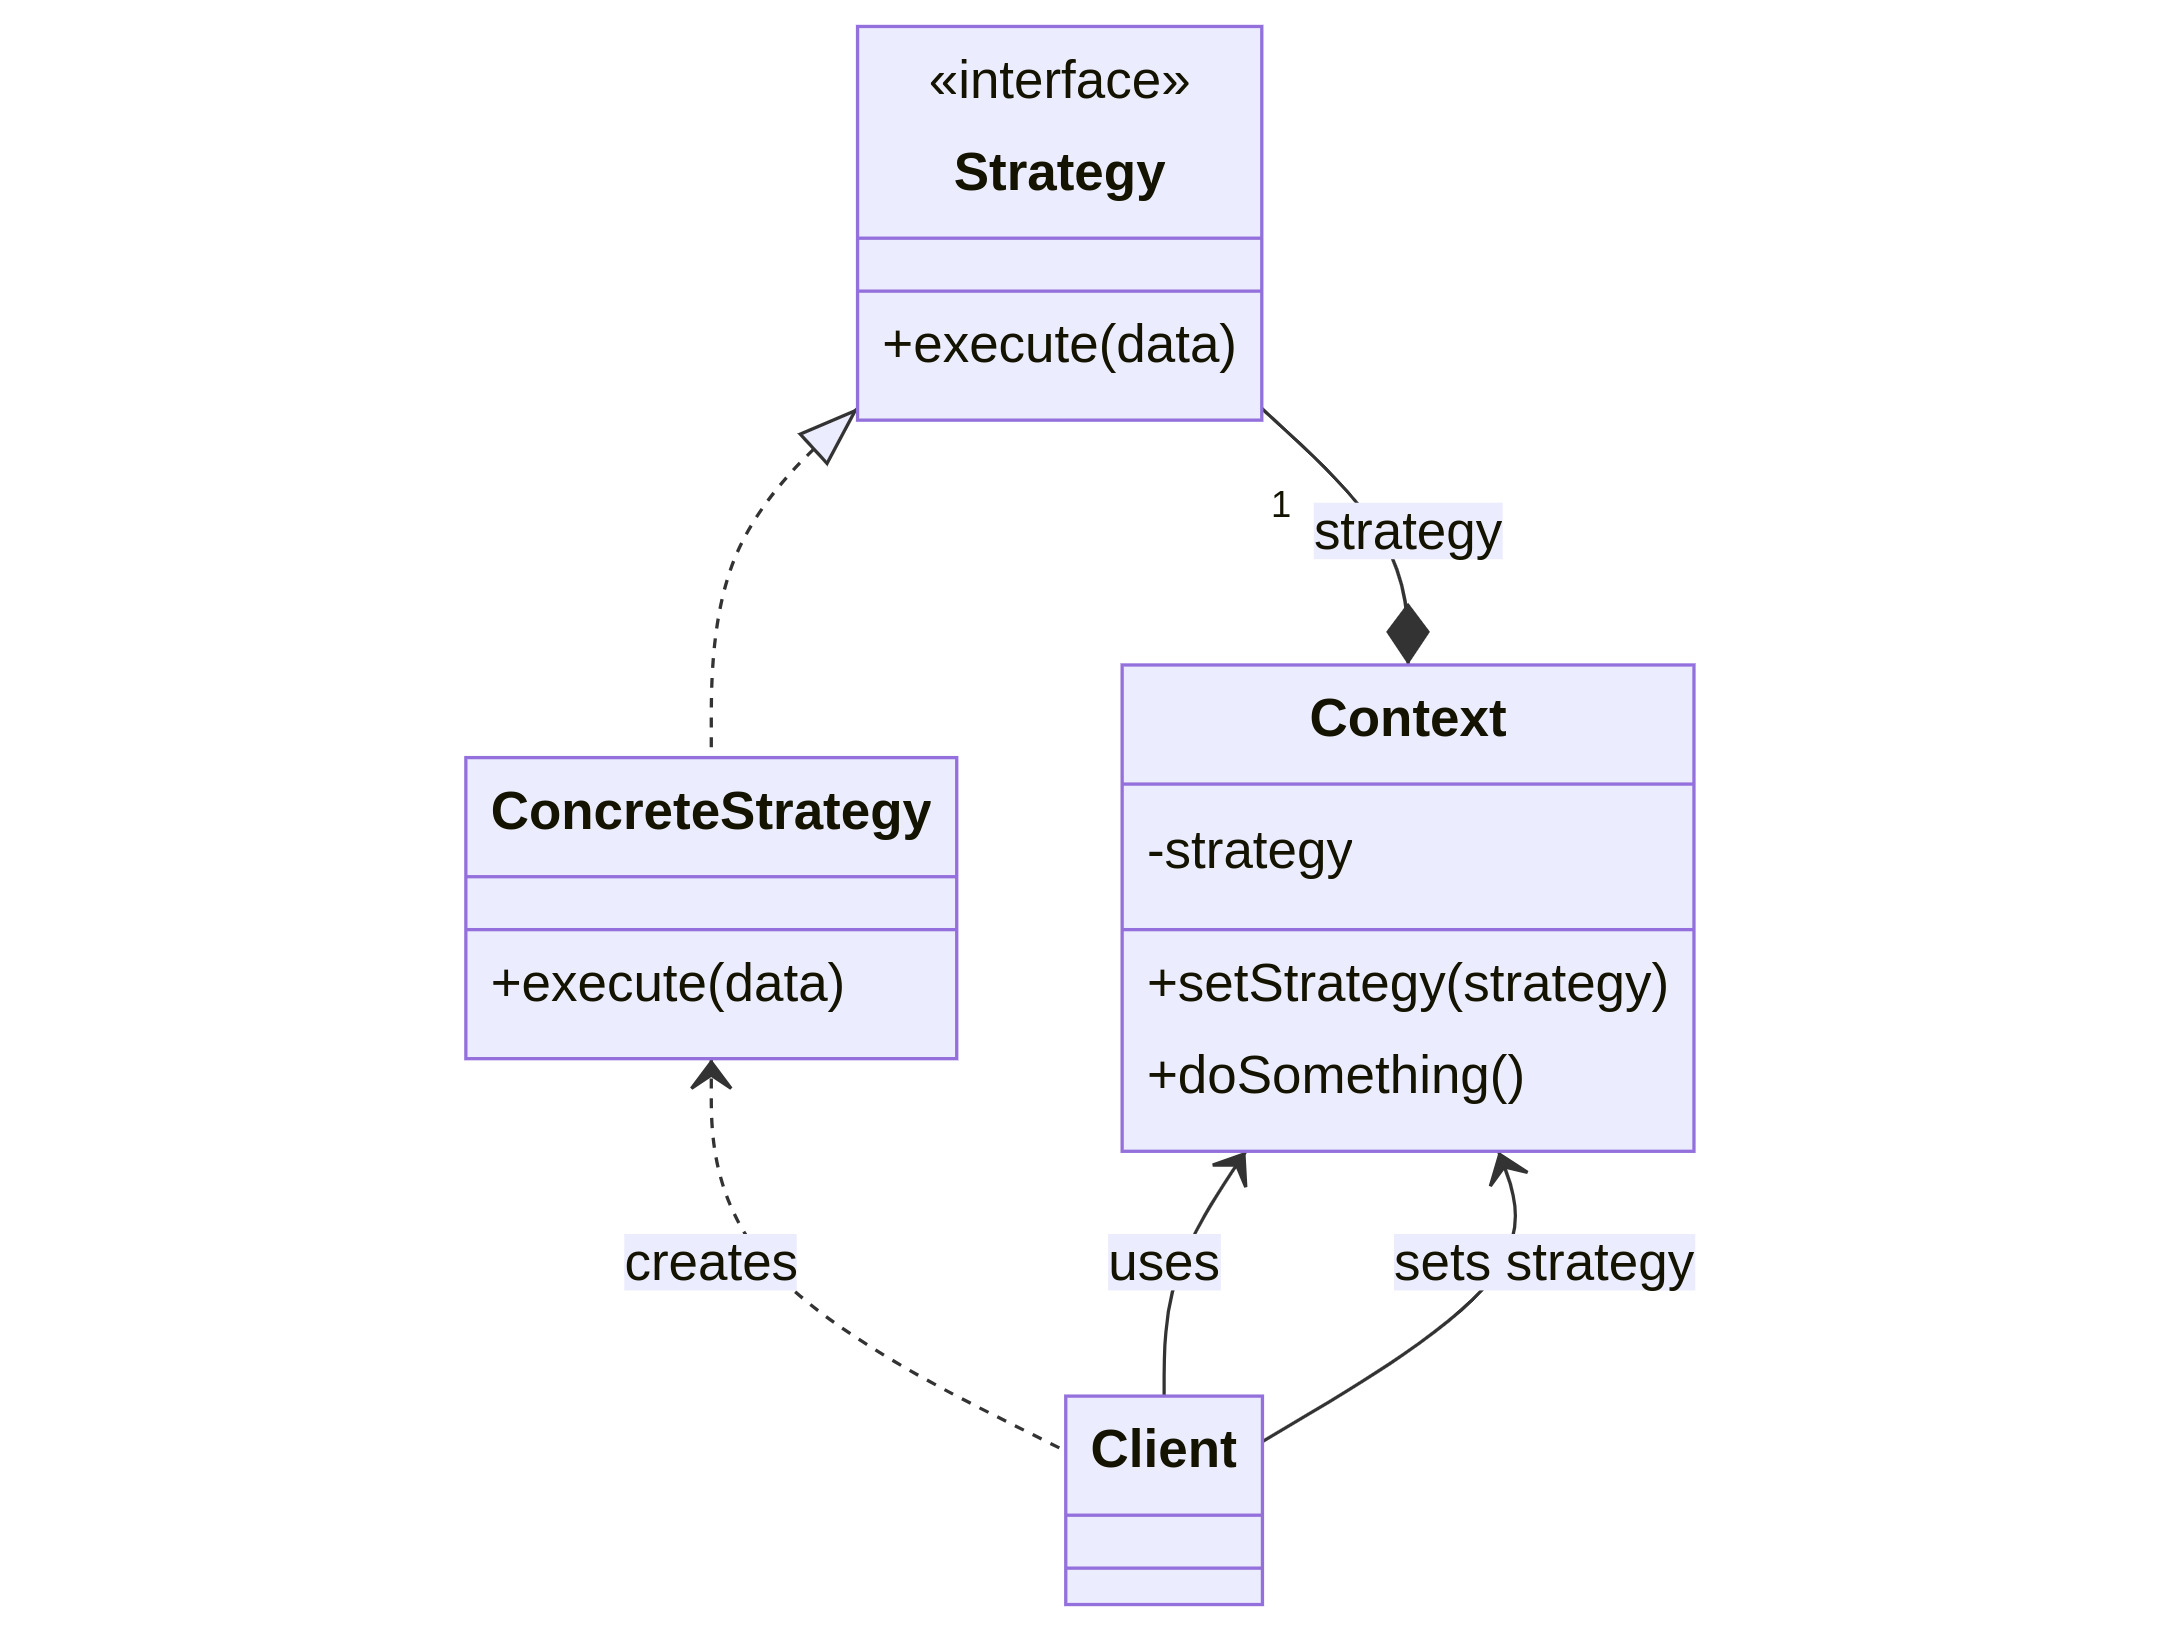
\includegraphics[width=0.75\linewidth]{images/patterns/strategy-class.png}
	\caption{Klassendiagramm des \emph{Strategy-Patterns}. \cite{skobeleva_strategy_2023}}
	\label{fig:strategy-class}
\end{figure}

Abbildung \ref{fig:strategy-seq} zeigt die typische Verwendung des \emph{Strategy-Patterns}. Der Kontext wird initialisiert, indem ihm vom Anwender eine konkrete Strategie zugewiesen wird (3), welche zuvor vom Anwender erzeugt wurde (1). Der Anwender kann von nun an den Kontext dazu veranlassen, eine Aktion durchzuführen, welche die Verwendung des in der hinterlegten Strategie vorhandenen Algorithmus nach sich zieht (5). Der Kontext kann den Algorithmus ausführen (6), ohne Wissen über die konkrete Strategie zu benötigen.

\begin{figure}[H]
	\centering
	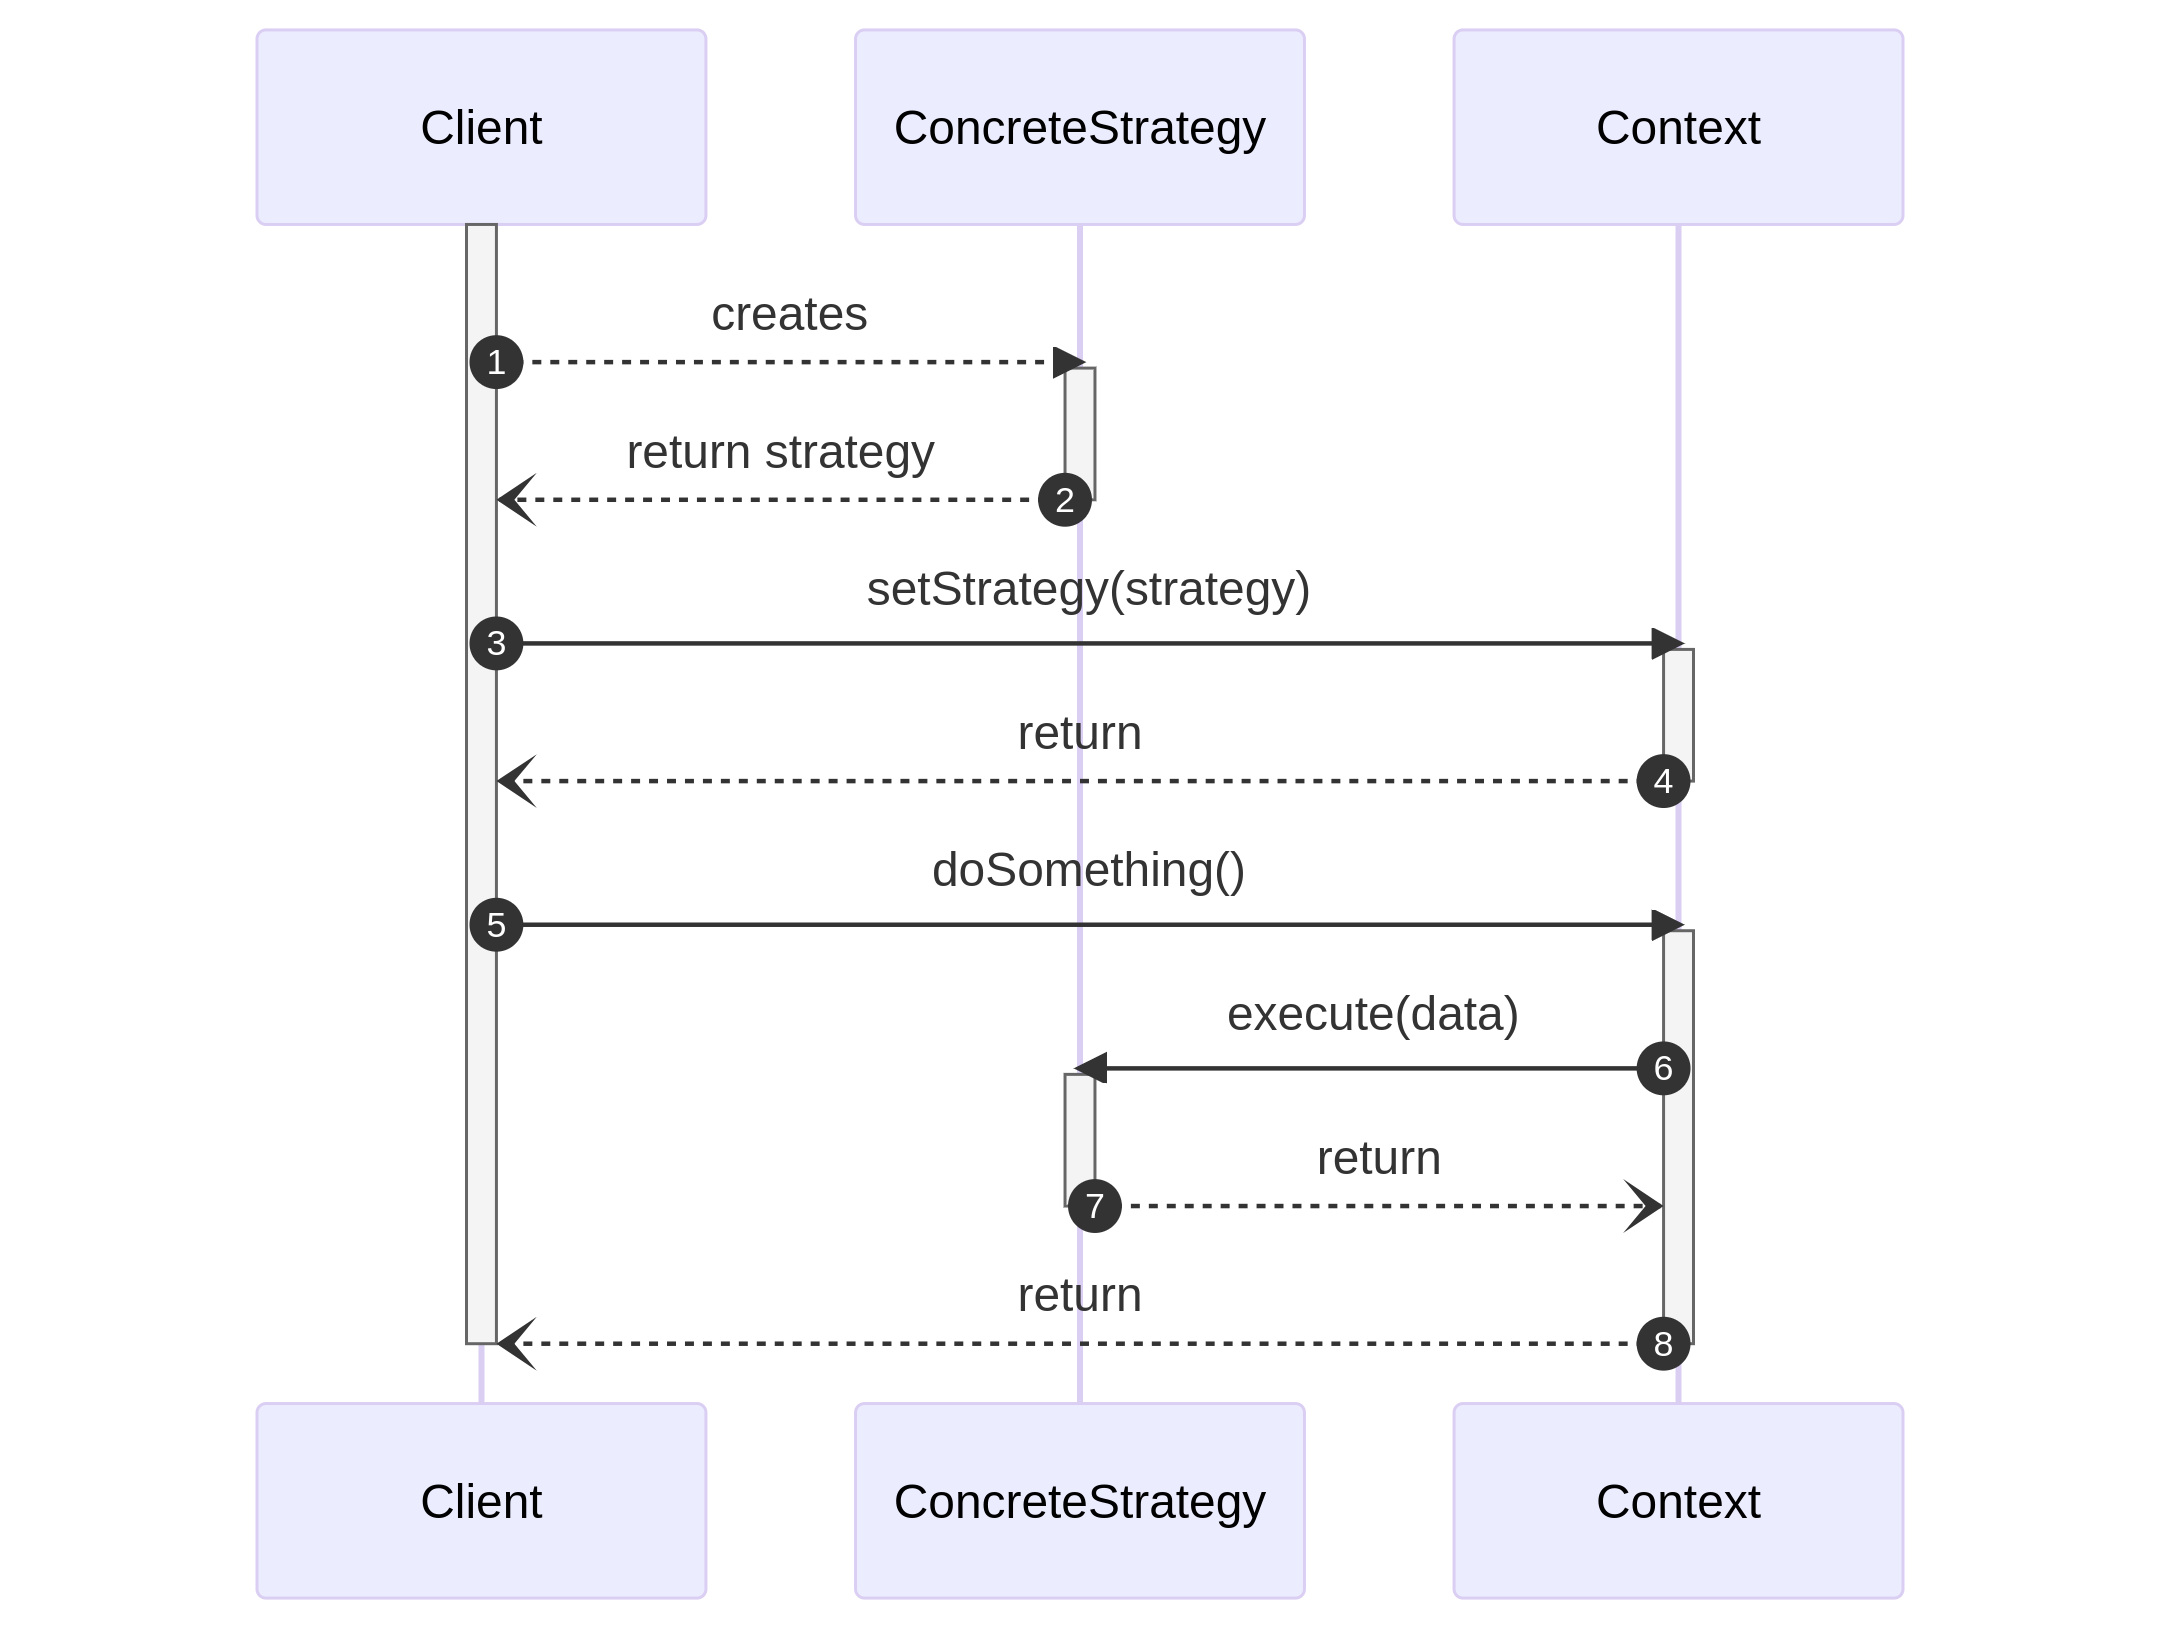
\includegraphics[width=0.75\linewidth]{images/patterns/strategy-seq.png}
	\caption{Sequenzdiagramm des \emph{Strategy-Pattern}. \cite{skobeleva_strategy_2023}}
	\label{fig:strategy-seq}
\end{figure}

\subsubsection*{Konsequenzen}
Das \emph{Strategy-Pattern} ermöglicht es, durch die Verwendung von Vererbung eine Hierarchie von Algorithmen aufzubauen. Das kann hilfreich sein, wenn mehrere Algorithmen sich Teile ihrer Implementierung teilen. Das Muster extrahiert die Algorithmen-Implementierung aus dessen Kontext und verhindert damit die sonst notwendige Bildung von Subklassen des Kontextes. Die Auswahl des auszuführenden Algorithmus wird über Aggregation gesteuert. Damit entfällt die Notwendigkeit von bedingten Sprüngen. Weiterhin können dank des \emph{Strategy-Patterns} auch mehrere Algorithmen bereitgestellt werden, deren Verhalten identisch ist und sich beispielsweise nur in der Performance unterscheiden. So kann je nach Laufzeitumgebung eine Entscheidung für eine bessere Laufzeit oder einen effizienteren Umgang mit Speicherressourcen getroffen werden.

Nachteile des \emph{Strategy-Patterns} sind zum einen ein erhöhter Mehraufwand für Kommunikation. Unter Umständen benötigt ein Algorithmus nicht die gesamte Schnittstelle, um zu funktionieren. Da der Kontext allerdings nur die abstrakte Schnittstelle der Strategie kennt, muss er stets die gesamte Schnittstelle bedienen. Das bedeutet unnötige Aufrufe von Methoden oder unnötige Übergabe von Parametern. Weiterhin erhöht dieses Muster die Gesamtzahl an Objekten und damit die Komplexität zur Laufzeit. \cite{gamma_design_1995}